\chapter{绪论}
\label{chap:introduction}

\section{研究背景与意义}
无人机集群系统(UAV Swarm Systems, USS)是一种模拟生物飞行系统工作原理而设计的新型仿生系统, 具有快速稳定、意志自适应以及集群涌现的工作优势。 集群的概念最早源自生物学研究, 表征个体间的间接协调机制。 这种协调机制表现为集群中的个体在无需任何集中规划和中心化通信情况下, 依靠个体间简单通信完成复杂群体活动的一种运行机制。 集群系统行为研究源于\citet{Flocks1987}等人提出的分离、聚集和速度一致三个基本规则(简称“Boids三原则”)。 基于Boids三原则, 个体通过相互之间的自主决策和简单信息交互, 经过演化最终使得整个群体在宏观上呈现出具有自组织、协作性和稳定性等整体行为特点。如图\ref{fig:swarm}所示, 经过个体之间的演化, 无人机集群系统可衍生出多种行为模式: 如无人机集群排列(Align)行为, 无人机集群聚集(Flock)行为和无人机集群组队(Group)行为等。

\begin{figure}
\centering
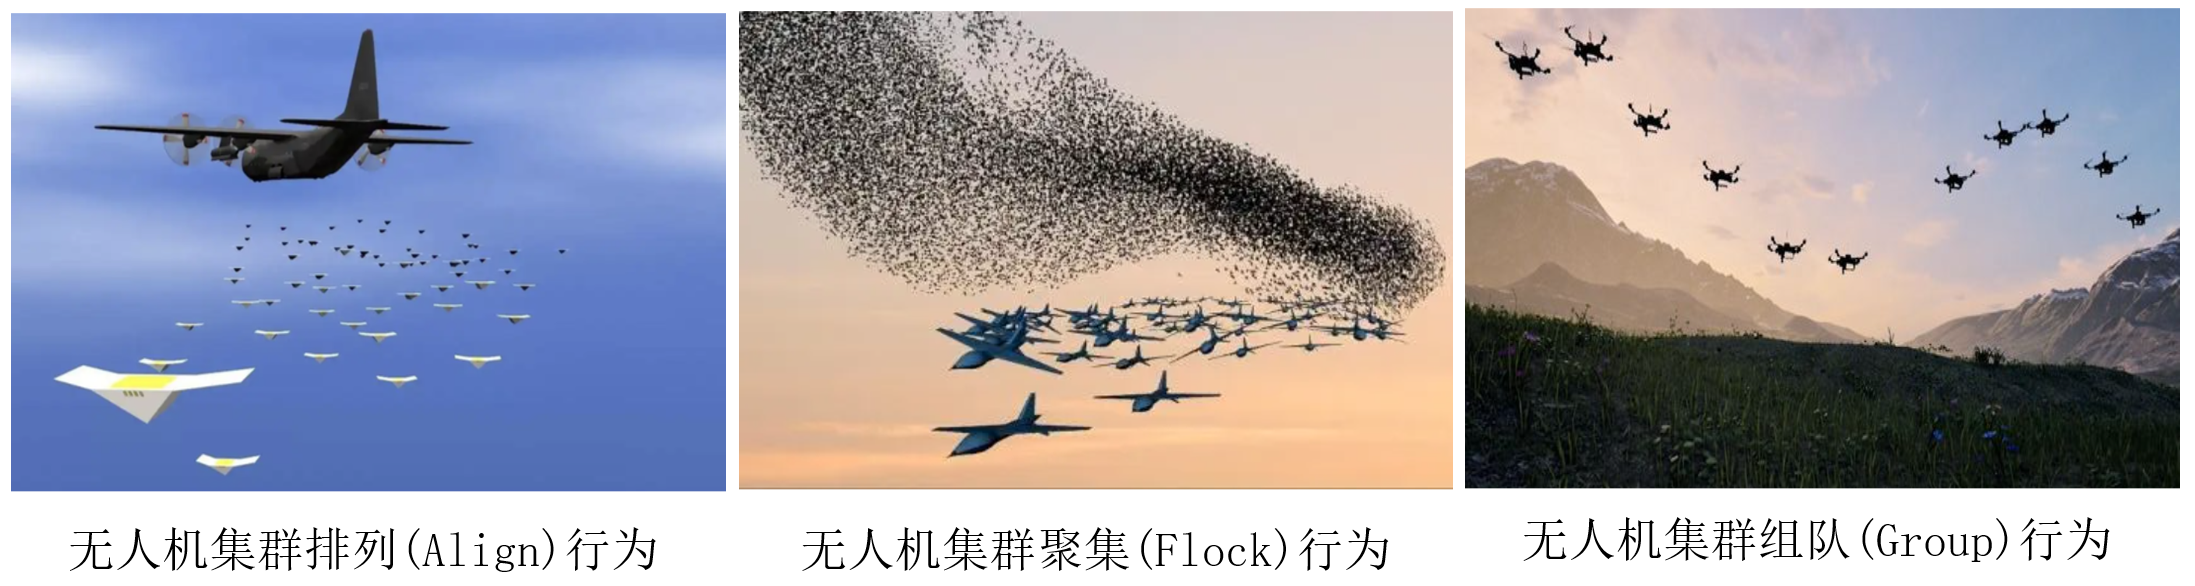
\includegraphics[width=1\linewidth]{Img/chapter0/swarm.png}
\caption{无人机集群若干典型行为示意图}
\label{fig:swarm}
\end{figure}

无人机集群系统在不同行为模式下可携带不同类型任务意图。通常而言, 无人机集群系统的行为与特定的任务分配具有一定的关联性, 对无人机集群行为的预判能够为无人机集群意图判别分析提供可用信息。例如, 在侦察任务下为躲避对方障碍物干扰, 无人机集群系统通常可采用排列(Align)行为; 在执行编队任务下无人机集群系统通常可通过聚集(Flock)行为或组队(Group)等行为模式达成任务目标。因此, 对无人机集群行为的分类研究可以为无人机集群意图推演和任务划分匹配提供前期的信息辅助, 是值得进行科研探索的方向之一。

无人机集群行为分类问题是指针对空中蜂群无人机整体行为的研究。当分布式无人机整体采取某种战略性和动态机动形式时, 无人机集群行为分类需要借助机器学习算法识别无人机集群行为模式并为未知无人机集群整体给出预测的行为类别\citep{Chung2018}。在先前的研究中, \citet{Hamann2018}提出针对无人机集群行为机器学习算法可以提供快速高效的分类结果。\citet{Brown2014}考察受限带宽约束条件下利用机器学习算法展开无人机集群行为分类。\citet{Brown2016DiscoveryAE}提出在单个无人机容量受限约束条件下利用机器学习算法开展集群行为分类问题。 \citet{Berger2016}提出降维算法将无人机集群行为数据压缩至低维线性子空间, 在低维线性子空间构建机器学习算法实现对无人机集群行为分类。 研究文献表明, 无人机集群相较于单个无人机可以完成更复杂的任务并且通过无人机集群的不同行为模式能够实现更丰富的目的意图推演\citep{Olaronke2020,Schranz2020}。 为此, \citet{Thomas2021}借助非线性时间序列预测模型探索无人机集群行为的特定对称性和动态特性之间的关系,并比较多种机器学习算法对于无人机集群行为预测效果。

\section{相关技术研究进展}
\subsection{无人机集群行为分类研究进展}
近些年的研究表明, 借助机器学习算法能够实现无人机集群行为分类。例如, 2014年美国空军动力研究院的\citet{Becker2014}采用压缩子空间学习技术结合机器学习算法实现无人机集群系统的行为判别。 他们将无人机集群整体的位置域信息和对应的无人机集群行为类别作为输入变量, 构建基于支持向量机模型的监督学习算法实现对无人机集群行为判别。\citet{Khan2020}于2018年提出采用混合人工判断的粒子行为判别实现无人机集群行为分类。 \citet{Hahn2019}在2019年提出采用增强学习理论进行无人机集群行为判别。2020年\citet{Lan2020}提出采用朴素贝叶斯, 高斯过程等统计学理论实现无人机集群行为分类。 

以上关于无人机集群行为分类的研究中, 大都基于无人机集群位置信息作为算法输入, 借用现代机器学习算法实现无人机集群行为分类。然而, 在许多机器学习算法应用中, 机器学习算法只会给出单值预测结果, 这种单值简单预测通常难以满足实际工程的需要。因此, 对机器学习算法输出结果给出可信程度的有效评估或者提供多类别输出的集合预测是非常重要的研究方向之一。

无论是对预测结果的可信评估还是集合预测, 这样的预测结果在理论上都属于对机器学习算法的不确定量化展开研究。对于许多风险敏感的科学研究领域, 例如医疗诊断\citep{Nouretdinov2013}、安全防卫\citep{Vineeth2014}及药物研发\citep{Janette2022}等领域, 给出机器学习输出结果的有效不确定量化预测是非常可取的。

主流学习算法中有两个主要领域可用于获得不确定量化研究, 分别是贝叶斯理论和“概率”近似正确理论(Probably Approximately Correct, PAC)\citep{Valiant1984}。 为应用贝叶斯框架, 需要具备一些关于数据生成的先验分布知识。 当有关数据分布的一些先验知识已知时, 贝叶斯方法可提供有效的最优决策。 然而, 对于经验推理科学\citep{Vapnik2006}并不具备有关分布的各种先验知识。 因此, 通常人们必须假设存在一个通用的规则, 进而在假设的通用规则下再展开问题的阐述。

历史上, 概率近似正确学习理论可以提供结果输出的不确定量化。 根据PAC学习模型, 首先预设犯错概率, 理论上要求保证在$1-\epsilon$概率下, 经验错误率小于等于$1-\epsilon$。 然而, 在具体现实研究中, 已有的结果已经表明, 概率近似正确理论下经验预测错误率边界往往远远超过$1-\epsilon$\citep{vovk2005algorithmic}。 同时, 概率近似正确学习理论对样本量需求巨大, 对噪声样本的容忍度较低, 模型的不确定量化结果鲁棒性较差\citep{vovk2005algorithmic}。 此外, 概率近似正确学习理论只能从整体上对预测的不确定进行评估和保证, 无法为每个样本提供不确定评估\citep{vovk2005algorithmic}。 因此, 基于概率近似正确学习理论的不确定量化, PAC学习理论通常无法得到有效保证\citep{Papadopoulos2008}。

对于其他传统概率预测算法, 如朴素贝叶斯(Na\"{i}ve Bayes)和逻辑回归(Logistic Regression)等传统统计模型, 其能够为每个个体预测结果提供不确定量化。 然而这些算法同样需要基于假设的概率分布展开。 然而严格说来, 传统统计和贝叶斯学习模型并不是“基于分布”展开数据分析, 而是“基于假设的分布”展开数据分析。 当数据符合假设的概率分布时, 贝叶斯学习的输出结果正确并且有效。 但如果数据不符合假设的概率分布, 尽管可以得到不错的预测结果, 但从理论上这些实用的结果大都无法得到有效保证的不确定量化结果\citep{vovk2005algorithmic}。

综上所述, 目前大多数机器学习算法仅仅给出预测结果, 但缺乏对预测结果提供有效不确定程度的考核。从理论角度审视这一问题, 即现有机器学习技术对每个预测结果无法提供有效的不确定量化\citep{2006Hedging}。

对于具有实际应用背景要求的无人机集群行为分类问题, 如何为机器学习算法的输出结果提供有效的不确定量化仍然面临着较大的挑战。在实际无人机集群行为分类研究中, 由于单一目的意图完全有可能采用多种无人机集群行为来实现, 因此有必要为无人机集群行为提供多类别集合预测。其次, 针对无人机集群行为分类问题, 由于真实数据本身的分布会随着时间发生变化, 基于前一种分布训练得到的学习模型难以继续为分布发生变化后数据提供高效预测, 因此有必要针对实际无人机集群数据提供一种有效的分布漂移检测\citep{Vovk2003,Vovk2012}。同时, 针对无人机集群数据稀缺的特点, 有必要开展小样本下无人机集群行为高效辨识研究\citep{Vapnik2009}。因此有必要针对上述科学问题开展研究。

\subsection{一致性预测方法研究进展}
Vapnik和Chervonenkis提出的统计学习理论提供一种基于纯粹数据驱动的无分布假设要求的新推理范式\citep{vapnik1974,vapnik1979,vapnik1982,vapnik1984,vapnik1995,vapnik1998,Vapnik2006,Chervonenkis2013}。 在这种新推理范式下, 通过控制两个因素(最小化经验风险泛函和诸函数的集合的容量)实现学习机器的构建。 统计学习理论是现象学学习模型\citep{Vapnik2019,Vapnik-context-2021,Vapnik-deep-2018,Vapnik-rethinking-2018}, 通过现象学还原\citep{vapnik2021-priviate-communication}可知学习机器的输出是一种暴力得分函数\citep{vapniktalk2015}, 不具备任何可信程度的度量\citep{2006Hedging}。 

一致性预测(Conformal Prediction, CP)是基于统计学习理论思想提出的一种无分布假设的可信机器学习解决方案\citep{vovk2005algorithmic}。 该算法框架由Vladimir Vovk, Alexander Gammerman和Glenn Shafer共同提出\citep{vovk2005algorithmic}, 它可以应用于任何学习算法之上来构建无分布假设的不确定度量。 与提供平均度量效果的传统统计方法不同, 一致性预测方法可以为单个个体提供有效的不确定度量指标。一致性预测提供置信度和可信度两种量化指标, 其中, 置信度衡量学习算法给出预测结果的可能性, 可信度衡量测试示例分类结果的适合程度。 与贝叶斯方法和PAC理论相比, 一致性预测方法给出的是有限样本下概率保证的有效不确定度量\citep{Poggi2017}。

一致性预测方法最初是在超越推理(Transductive Inference)范式\citep{vovk2021-priviate-communication}为机器学习算法的预测结果提供可靠评估的一套框架\citep{gammerman1998,soton1999,Saunders1999}。 基于柯尔莫哥洛夫概率论\citep{Kolmogorov1933,Kolmogorov-en-1956}, 在柯尔莫哥洛夫算法复杂度基础上\citep{Kolmogorov-en-1931-analytical,Kolmogorov-en-1946-leastsquare,Kolmogorov-en-1983,Kolmogorov-en-1991,Heidegger1966}结合Vapnik提出的支持向量机理论\citep{Cortes1995,vapnik1998}, Vovk将支持向量机理论中的支持向量的概念转译为置信预测, 这样在理论上就可以基于对冲预测提供一种可信赖的统计推断\citep{vovk2005algorithmic,2006Hedging}, 即对于给定训练数据集和新的观测数据, 可以基于一致性预测构建预测目标的置信区间。

采用一致性预测算法, 可以解决机器学习这类黑箱算法预测的不确定量化等科学问题。 传统机器学习算法是能够实现集群行为分类任务的, 其分类准确性度量一般建立在对测试数据预测能力的总体考核上, 其通用的评估方式(如均方误差类指标)大都采用对测试数据的平均汇总误差来表征算法的预测性能。 通用方法无法为单个样本的预测表现提供量化评估。 然而, 对于无人机集群行为判别这类高风险、低容错的研究任务需求, 采用常规意义上的整体误差评价指标无法为这类实际工程提供充分的不确定量化信息支持。 因此, 在本研究中需要考虑为无人机集群的单个预测输出提供有效的不确定量化, 并基于此实现机器学习黑箱算法的不确定量化。 

一致性预测是很有弹性的算法框架, 可以将一致性预测视为一种“刷子算法”, 任何机器学习算法经过改造都可以作为一致性预测的底层算法。 一致性预测算法能够对底层算法的输出“刷”上不确定量度, 并且其提供的不确定度量的有效性可以从理论上自动得到保障。 一致性预测成为学习理论的一个新方向并且是统计学习理论研究中的一种新的范式\citep{2006Hedging}, 因为一致性预测提供的不确定量度是基于有限样本的断言, 其不会考虑任何渐近的应诺式解决方案\citep{vovk2005algorithmic,2006Hedging}。

%
%一致性预测针对具体应用背景的特点, 结合统计学习理论为机器学习算法输出展开校正。 一致性预测对机器学习系统的预测结果提供可靠性评估和保障。 这种学习算法框架的优越性体现在如下几个方面: 首先, 一致性预测在对机器学习算法输出的每个个体的预测结果可以提供可靠性评估的同时能够确保整体预测结果的可靠性。 其次, 一致性预测框架提供的可靠性评估是有效的。 有效性是这一算法的重要性质。 再者, 一致性预测能够为任何机器学习算法提供有效的不确定度量。 特别重要的是, 区别于传统统计学总是基于渐近意义下得出的应诺(assure), 与之相反, 一致性预测的有效性不依托于渐近理论, 其阐述的有效性是在有限样本下给出的断言(assert)。 正是由于传统统计学算法无法提供有效估计, 这使得一致性估计在近几年越来越受到数据科学领域研究人员的关注。 

一致性预测在时间序列分析, 模式识别和回归分析领域都有大量的应用研究\citep{Vineeth2019}。\citet{Lei2015}提出采用一致性预测处理泛函数据分析任务, 并且给出无分布假设的统计推断方法。 \citet{Vovk2021retrain}提出使用一致性预测检测学习机器泛化推广能力的边界。\citet{Aleksandrova2021}通过大量实证研究说明一致性预测提供完整有效的不确定量化研究框架, 是解决现代机器学习不确定量化的重要研究方向。\citet{Victor2018}针对相依数据展开一致性预测研究, 提出一致性预测对于相依数据也能够提供精确的不确定量化结果。\citet{Xu2021}提出采用一致性预测算法为动态时间序列数据提供区间估计并且给出可行的解决方案。\citet{Dashevskiy2011}利用一致性预测方法为时间序列分类给出可信赖的预测。\citet{Papadopoulos2007}为神经网络提供一整套完整的基于一致性预测的不确定量化框架\citep{Papadopoulos2008}。\citet{Janette2022}提出针对临床医疗科学采用一致性预测方法提供不确定量化。

\subsection{分布漂移检测方法研究进展}

一致性预测的主要不足之处在于其前提建立在数据满足独立同分布假设上\citep{Finetti1975}。 在机器学习实际应用中, 研究者大都会随机将数据采样为训练集和测试集, 这样技术层面的操作一方面使得在建模时所用数据符合独立同分布假设的要求, 另一方面通过随机化采样数据使得训练模型在处理后数据上表现出相当优越的泛化学习推广能力。 然而在某些特定领域由于数据资源本身的稀缺特点以及研制问题本身的要求, 这就使得在需要面对数据本来的顺序时, 一致性预测的效率有所降低。

在处理实际应用问题时, 由于无法提前随机化数据, 数据的分布会随着时间发生变化。因此, 有必要给出关于数据本身分布的漂移检测度量标准。 分布漂移检测是统计学研究的重点, 但是仔细考察就会发现统计学将这一问题巧妙地归约为处理假设分布的漂移检测问题。 然而对于实际工程中的数据分析任务, 研究者通常并不能先验地给出任何关于分布的假设。 因此, 传统统计学给出的方法就始终扭结在到底如何提供很好的分布假设这一困境中\citep{Breiman2001,Efron2020}。

为解决上述问题, \citet{Vovk2003,Vovk2021retrain}提出一种无分布假设的分布漂移检测理论。根据此理论, 可以在各种应用背景下展开对研制问题数据本身分布的漂移检测。例如, \citet{Ho2005}使用此方法解决时变数据流的异常检测问题; \citet{Ho2012}应用鞅序列检测方法为高维时变数据流的可交换性提供一种端到端的解决方案; \citet{Ho2019}则将鞅序列方法应用于飞行轨迹的异常检验问题。 \citet{Vovk2012}提出一种基于“Plug-In”方法的分布漂移检测理论并将之应用于解决实际问题中的分布漂移检测。 这些实际的应用都已经表明采用无分布假设的分布漂移检测理论能够为实际问题提供优质的解决方案。 然而, 在无人机集群行为分类问题中还没有文献关注集群行为分类任务中分布漂移检测问题。 


\citet{Vovk1993}提出这种无分布假设的分布漂移检测方法利用机器学习的输出来实现对数据本身分布的检测。这种方法首先需要根据机器学习算法的输出构建鞅序列。而根据Vapnik-Chervonenkis理论, 机器学习算法属于现象学学习模型, 这种学习模型无需任何分布假设。 因此, \citet{Vovk1993}提出检测方法可以直接地检测“数据本身的分布漂移”, 而并不是检测“假设的分布漂移”。

综合目前研究结果和无人机集群研究的现实需要, 本文提出一种无分布假设的分布漂移检测方法, 这种方法能够为超高维数据提供端到端的分布漂移检测方案。这种方法无需任何先验知识, 仅仅依靠底层学习算法的输出, 构建得到的鞅序列即可完成分布漂移检测任务。 因此这种方法对于处理复杂无人机集群行为问题提供一种全新的分布漂移检测和预报方案。


\subsection{使用特权信息学习方法研究进展}

以上研究内容中所提出的方法都建立在机器学习算法的输出而展开。因此, 上述研究都依赖于底层机器学习算法的数据压缩能力。不难发现, 现有机器学习算法大都建立在大样本基础之上。然而, 考虑到无人机集群问题的实际应用背景, 有必要开展在小样本下的机器学习算法研究。

使用特权信息学习(Learning Using Privileged Information, LUPI)是机器学习领域中具有里程碑式的一种新学习范式\citep{Vapnik2009}。这种学习范式使得在机器学习领域能够提供直观学习\citep{Lerner1972,Ewald1996-1,Ewald1996-2}, 并且提供一种在小样本下的确保达到高精度的预测算法。特权信息的特点是其只能在训练阶段可用而在测试阶段不可用, 并且有效的特权信息需要研究者对所研问题提供整体描述信息\citep{Vapnik2006}。根据LUPI理论证明, 采用LUPI算法能够明显加速学习算法的收敛速度, 使得小样本下获得高精度的预测效果成为可能\citep{Pechyony2010}。

近些年, 使用特权信息学习模型在很多实际应用领域中得到广泛关注。 例如在特征选择研究中, \citet{Izmailov2018}基于$L_{1}$范数稀疏约束的LUPI范式下构建特征选择分类器。基于LUPI范式的特征选择能够扩充训练阶段的特征尺度, 从而显著提升机器学习算法的预测性能。为解决人机交互中潜变量的获取, \citet{Vrigkas2017}提出利用LUPI算法构建现代人机交互学习模式, 将研究者提供的直观信息输入学习算法来增强模型的稳定性。 在\citet{Vapnik-similary-2015}的工作中, Vapnik提出更新后的LUPI算法, 这种算法通过特权信息控制学习机器的容量从而加速学习算法的收敛。 \citet{Lapin2014}将LUPI算法的思想纳入SVM+框架, 同时引进二次优化算法实现所研问题的求解。 在许多实际应用问题研究中, 作者提出一种基于LUPI的问题求解器处理各种实际问题。 例如, \citet{Li2016}提出基于SVM+的特权信息模型解决各种预测和模式识别问题。\citet{Zheng2017}将LUPI框架应用医学影像诊断来实现小样本下高效分类的目标。

\section{研究内容与安排}
基于以上研究背景和技术进展状况, 从提高无人机集群行为分类的可信赖机器学习出发, 本文对无人机集群可信行为分类, 无人机集群分布漂移检测和小样本下无人机集群高精度分类设计进行研究。论文共分为\ref{chapter:conclusion}章。第\ref{chap:introduction}章是全文的背景介绍和问题引出。第\ref{chap:edbed}章是全文的理论基础。第\ref{chap:Swarm-MCP}章展开的是无人机集群行为分类的可信机器学习研究, 针对机器学习算法提出一种有效的不确定量化。第\ref{chapter:swarm-distributions}章和第\ref{chapter:swarm-martingales}章是针对无人机集群行为数据分布漂移相关内容展开的研究。针对无人机集群行为数据本身的分布随时间发生变化的现实, 本文研究如何在无分布假设的要求下开展分布漂移检测。针对检测到的分布漂移信息, 本文提出采用鞅保护分布算法来增强底层学习算法的预测性能。第\ref{chap:intelligent-learning}章是为小样本下无人机集群行为分类提出一种全新的学习范式。在小样本训练要求下, 本文提出使用特权信息学习方法加速学习算法收敛, 使得在无人机集群行为分类中通过提供整体描述实现小样本下高精度预测。第\ref{chapter:conclusion}章为总结与展望。本文研究框架如图\ref{fig:thesis-frame}所示, 在研究框架图中单列每一章节研究的主题词, 各章主要内容如下:

\begin{figure}
\centering
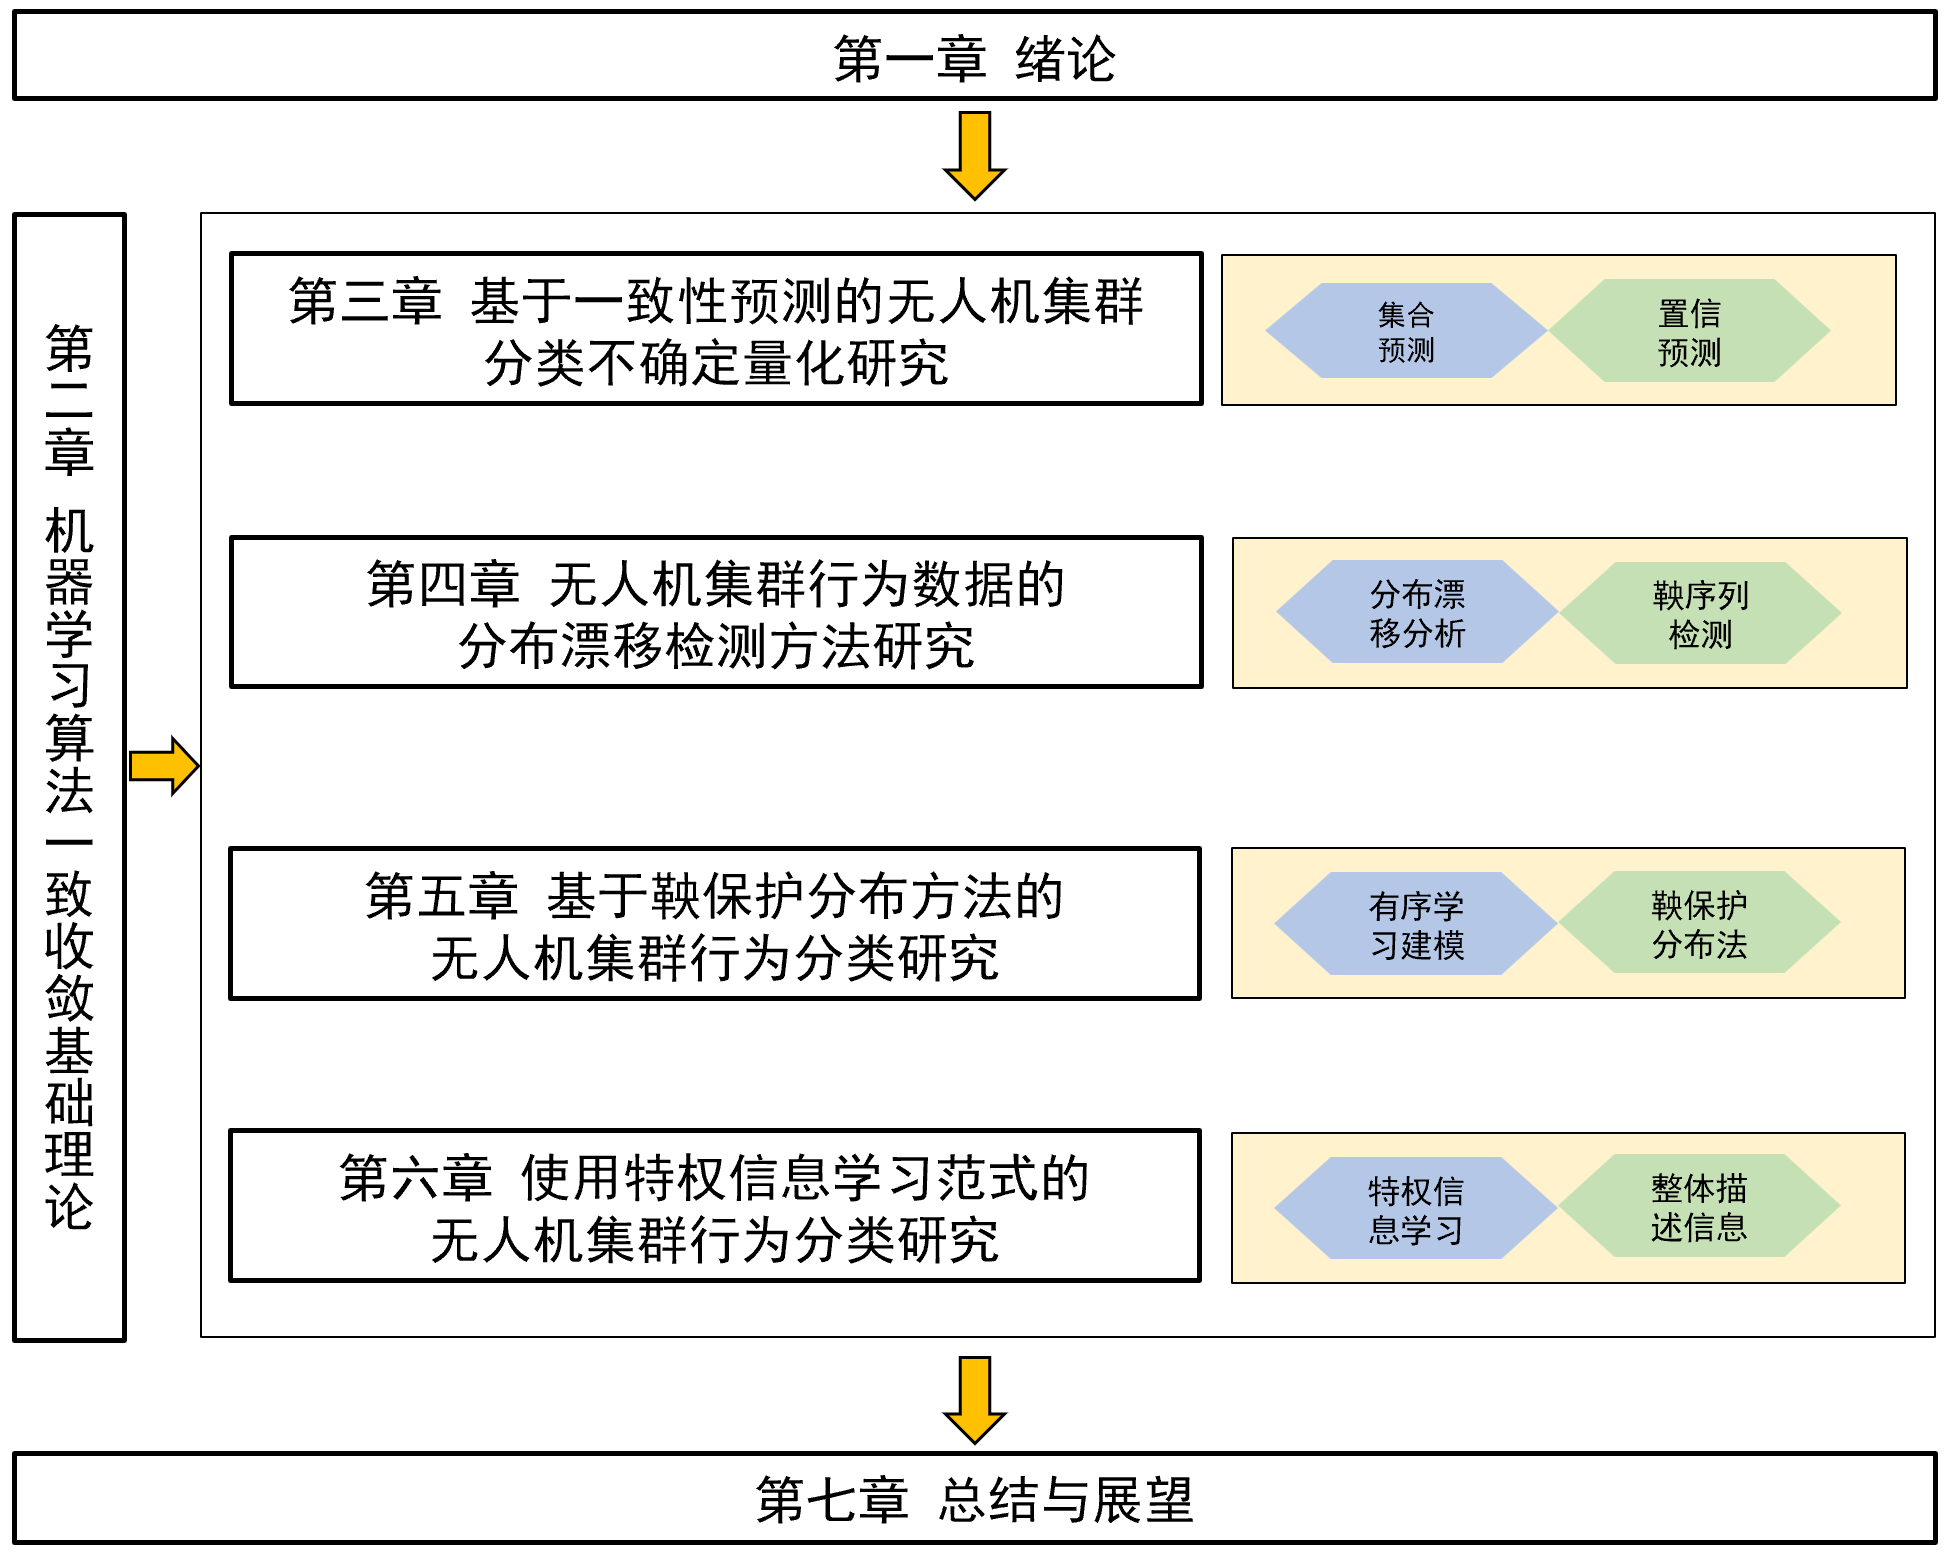
\includegraphics[width=.9\linewidth]{Img/thesis-frame}
\caption{论文组织结构图}
\label{fig:thesis-frame}
\end{figure}

第\ref{chap:introduction}章, 绪论。首先介绍论文的研究背景与意义, 然后从一致性预测方法、分布漂移检测方法和使用特权信息学习三个方面概述现有方法的研究进展。

第\ref{chap:edbed}章, 介绍统计学习理论基础, 着重强调机器学习算法的现象学学习模型基础。本文指出需要控制两个因素: 其一是经验风险最小化, 其二是学习机器的容量来使得学习问题的一致收敛条件成立。根据统计学习理论可知, 以上控制学习问题收敛的两个因素唯一受VC维的控制。 因此, 在后续实际应用中要始终围绕如何控制容量展开研究, 并且突出强调Vapnik-Chervonenkis理论给出的关于学习理论的阐述是一种断言式的解答而不是应诺式的言说。由于本文的工作都在机器学习算法的顶层展开, 因此得出的结论都是有保证的可信赖推理结果。

第\ref{chap:Swarm-MCP}章, 在一致性预测的基础上提出改进后的蒙德里安一致性预测为复杂无人机集群行为的可信分类提供精确有效的统计推断。 本文为无人机集群行为分类提供两种精确有效的可信预测模型, 其一是精确有效的置信预测, 即为当前机器学习简单预测结果给出精确有效的置信度度量和可信度度量; 其二, 为复杂无人机集群行为分类提供一种精确有效的有保证的集合预测。 与此同时, 针对每一种预测结果本文都检验预测结果的有效性, 这些精确检验算例验证所提方法的可行性和有效性。

第\ref{chapter:swarm-distributions}章, 在一致性预测基础上开展无人机集群分布漂移检测研究。 本文注意到构建常规机器学习算法时一般默认将整个数据集随机采样得到训练集和测试集合, 然后用训练集训练机器学习算法并在测试集合上检验此算法的预测效果。根据现代概率论相关知识, 借助技术随机化经验数据能够使得处理数据满足模型前提假设, 但同时会消除数据本身的某些重要的分布信息。 为此本文提出一种无分布假设的鞅序列方法检测数据本身的分布信息。所提方法是在机器学习算法输出结果之上展开的, 是一种能够处理超高维数据、无任何分布假设先验要求的分布漂移检测方法, 能够对分布漂移检测问题提供端到端的高效检测。最后,通过真实无人机集群行为数据集验证所提方法的可行性和有效性。

第\ref{chapter:swarm-martingales}章, 通过采用鞅保护分布方法将鞅检测理论与机器学习算法相结合, 并提出利用鞅保护分布理论改进底层学习算法的完整框架。将鞅保护分布算法纳入考量之后, 真实数据的分布漂移信息就可以加入训练模型, 因此本文提出的算法能够增强原先学习算法的泛化推广能力。 本文将提出的鞅保护分布算法应用于多种机器学习算法之上, 通过三种公开的真实无人机集群行为数据集分别测试所提出的算法。试验结果证明, 所提方法对各类底层机器学习算法大都具有显著的提升, 同时也验证所提鞅保护分布算法的可行性和有效性。

第\ref{chap:intelligent-learning}章, 提出一种新的学习范式(即使用特权信息学习)处理小样本下无人机集群行为分类问题。特权信息是在训练阶段可用, 但是测试阶段不可用的整体描述信息。首先, 选取无人机集群中个体间合作描述信息作为特权信息, 阐述在合作描述信息作为特权信息模型下, 无人机集群行为分类实现小样本训练而达到高精度预测能力的模型。其次, 选取无人机集群个体间竞争描述信息作为特权信息, 阐述在竞争描述信息作为特权信息模型下, 无人机集群行为分类实现小样本训练而达到高精度预测能力的模型。本文将这两种模型分别应用于三种公开无人机集群行为数据, 分别检验特权信息在三种无人机集群行为数据集下的预测效果, 试验结果证实所提基于特权信息学习模型方案的可行性和有效性。

第\ref{chapter:conclusion}章对全文内容进行总结并给出进一步研究的展望。